\documentclass[10pt]{beamer}

%\usetheme{Montpellier}
\usetheme{Madrid}

\usecolortheme{beaver}
\usepackage{appendixnumberbeamer}
\usepackage[utf8]{inputenc}
\usepackage[spanish]{babel}
\usepackage{booktabs}
\usepackage[scale=2]{ccicons}
\usepackage{pgfplots}
\usepackage{framed}
\usepgfplotslibrary{dateplot}
\usepackage{xspace}
\usepackage{csquotes}
\usepackage{graphicx}
\usepackage{verbatim}
\usepackage{listings}

\newcommand{\themename}{\textbf{\textsc{metropolis}}\xspace}
\graphicspath{ {images/} }


\title{Estratificación temporal de Aedes Aegypti basada en herramientas geoespaciales y aprendizaje automático}
%\subtitle{Trabajo Final de Grado, Licenciatura en Ciencias de la Computación}

\date{Diciembre de 2018}

\author{Juan M. Scavuzzo}
\institute{Facultad de Matemática, Astronomía, Física y Computación \\ Universidad Nacional de Córdoba}
\begin{document}

\maketitle



\begin{frame}{Motivación de este trabajo: problemática epidemiológica}
  \begin{itemize}[<+->]
   \item Aedes aegypti es el principal vector de Dengue, Chikungunya, Zika
         y Fiebre Amarilla urbana
   \item Datos de la Organización Mundial de la Salud:
    \begin{itemize}[<+->]
      \item 80 millones de personas se infectan de Dengue anualmente
      \item 550 mil enfermos requieren hospitalización
      \item 20 mil personas mueren
      \item 2.500 millones de personas corren riesgo de contraer la enfermedad
      \item Más de 100 países con transmisión endémica
    \end{itemize}
  \end{itemize}
\end{frame}



\begin{frame}{Motivación de este trabajo: problemática epidemiológica}

  \begin{center}
    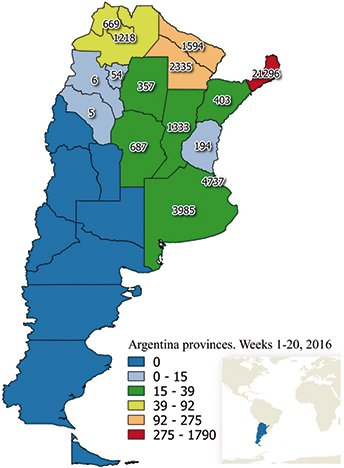
\includegraphics[width=0.4\textwidth]{dengue}
  \end{center}

\end{frame}



\begin{frame}{Motivación de este trabajo: problemática epidemiológica}
  Características del Aedes aegypti
  \pause
  \begin{itemize}[<+->]
   \item Gran capacidad adaptativa
   \item Resistencia a insecticidas
   \item Resistencia de huevos a la desecación
   \item Presencia en el medio urbano
   \item Preferencia de cria en contenedores artificiales
  \end{itemize}
\end{frame}



\begin{frame}{Motivación de este trabajo: sistemas de modelado actuales}
  Modelar utilizando información satelital
  \pause
  \begin{itemize}[<+->]
   \item Información ambiental con alcance regional
   \item Información espacio-temporal
   \item Grandes avances en los últimos años
   \pause

  \end{itemize}
  \begin{center}
    Pero actualmente se utilizan modelos lineales para relacionar las distintas
    variables!
  \end{center}

\end{frame}



\begin{frame}{Motivación de este trabajo}
  Algunas cuestiones a tener en cuenta
  \pause
  \begin{itemize}[<+->]
   \item La prevención de las enfermedades en cuestión debe ser a través de control de vectores
   \begin{itemize}
     \item Modelos predictivos!
   \end{itemize}
   \item Será correcto asumir relaciones lineales entre las variables ambientales y la abundancia del vector?
   \begin{itemize}
     \item Modelos no-lineales con... aprendizaje automático!
   \end{itemize}
   \item Si es un sistema regional, cómo extrapolo los modelos?
   \begin{itemize}
     \item A través de relaciones entre características ambientales!
   \end{itemize}
  \end{itemize}

\end{frame}


\begin{frame}{Objetivos}
  \pause
  \begin{itemize}[<+->]
   \item Implementar una herramienta, sencilla, para generar modelos predictivos
   \item Validar la hipótesis de que "modelos no-lineales son mejores para predecir la oviposición que los lineales"
   \item Proponer una solución a la problemática de escases de datos que se evidencia al pensar en sistemas regionales de estimación de riesgo

  \end{itemize}

\end{frame}


\begin{frame}{Algunos Conceptos: \textit{Epidemiología Panorámica}}
  \begin{center}
      Algunos conceptos importantes
  \end{center}

\end{frame}


\begin{frame}{Algunos Conceptos: \textit{Epidemiología Panorámica}}
  \pause
  \begin{itemize}[<+->]
   \item La teledetección y su capacidad de adquirir información
   \item Información sobre hábitat de insectos y artrópodos
   \item Fuente de datos sobre la distribución espacio-temporal de enfermedades
         transmitidas por vectores (Pavlovsky)
  \end{itemize}

\end{frame}


\begin{frame}{Algunos Conceptos: \textit{Epidemiología Panorámica}}
  \begin{center}
    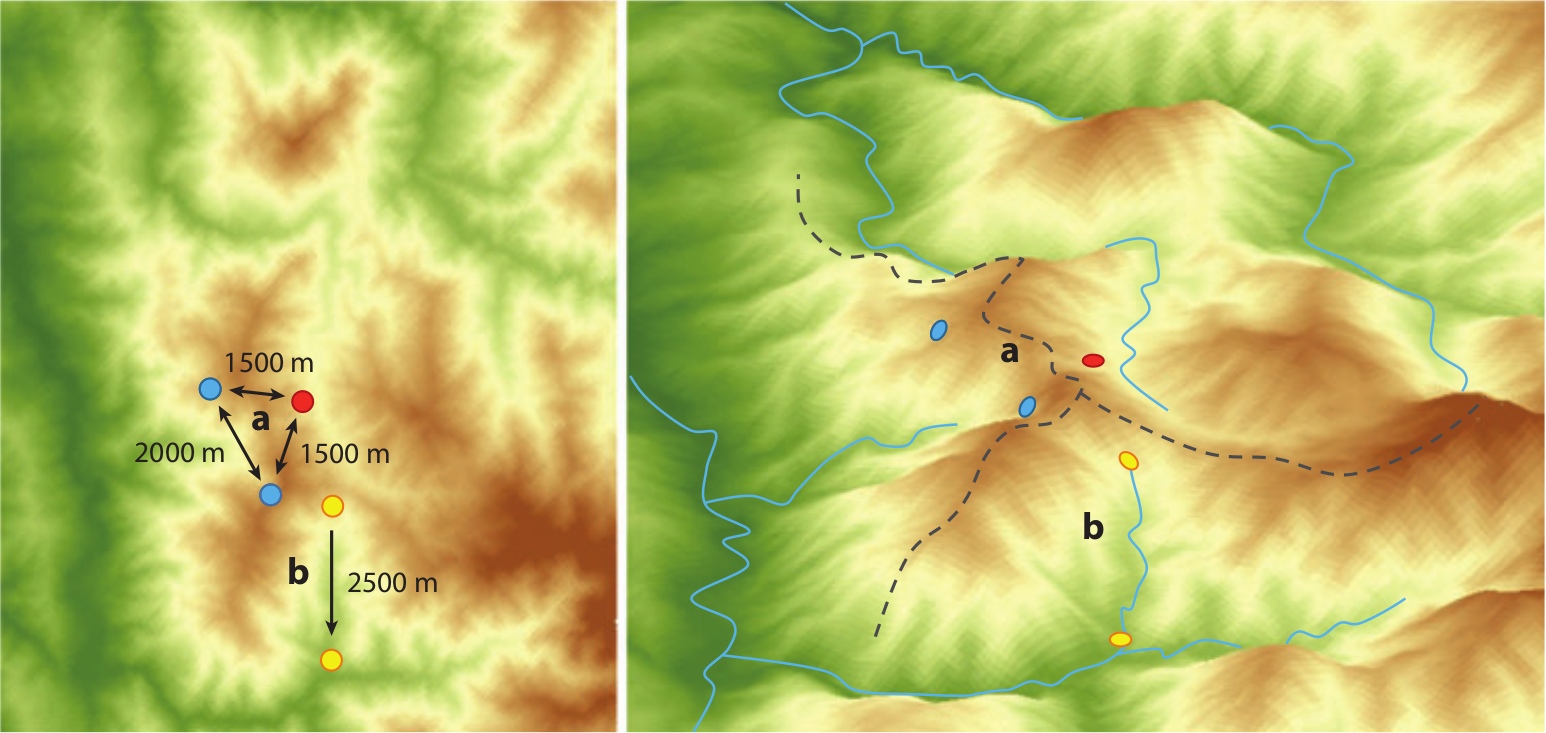
\includegraphics[width=1\textwidth]{paisajes_heterogeneos}
  \end{center}
\end{frame}



\begin{frame}{Algunos Conceptos: \textit{Epidemiología Panorámica}}
  \begin{itemize}[<+->]
   \item Ecología panorámica
   \item Focalidad
    \begin{itemize}
      \item Vectores con capacidad de transmisión de la infección
      \item Vertebrados capaces de funcionar como reservorio de la infección
      \item Huéspedes susceptibles, como humanos o animales domésticos
    \end{itemize}
    \pause
  \end{itemize}
  \begin{center}
    \textbf{\textit{Epidemiología Panorámica}}
  \end{center}
\end{frame}


\begin{frame}{Algunos Conceptos: \textit{Aprendizaje automático}}
  \begin{framed}
    \begin{center}
      \textit{Se dice que un programa de computadora \textbf{aprende} de experiencia
      $E$ con respecto a alguna tarea $T$ y una métrica de rendimiento $M$, si
      con la experiencia $E$ se incrementa su rendimiento en la tarea $T$,
      medida por $M$.}\\
    \end{center}
    \centering \textbf{Tom Mitchell, 1997} \cite{mitchell_learn}
  \end{framed}

\end{frame}



\begin{frame}{Algunos Conceptos: \textit{Aprendizaje automático (ML)}}
\begin{itemize}
  \item Enfoque empírico efectivo para \textit{regresiones} y \textit{clasificaciones}
  \item Distintos métodos:
    \begin{itemize}
      \item Supervisados: Regresiones Lineales, SVMs, ANNs, DTRs...
      \item No-supervisados: K-NNs, K-means, PCA...
      \item Semi-supervisados
    \end{itemize}
  \item Usado en muchos ámbitos:
  \begin{itemize}
    \item Académico
    \item Industrial
    \item Gubernamental
  \end{itemize}

\end{itemize}
\end{frame}



\begin{frame}{Algunos Conceptos: \textit{Métodos Supervisados}}
\begin{itemize}
  \item Aprenden a través de pares de ejemplos $(X, Y_{verd})$
  \item Conjuntos de entrenamiento y validación
  \item Evitar \textit{overfitting}
  \item Ajuste de hiperparámetros...
\end{itemize}
\end{frame}

\begin{frame}{Algunos Conceptos: \textit{Parámetros y Hiperparámetros}}
  \begin{itemize}
    \item Los algoritmos de ML poseen \textit{parámetros} e \textit{hiperparámetros}
    \begin{itemize}
      \item Los hiperparámetros definen el comportamiento durante el proceso de entrenamiento
      \item Los parámetros se ajustan para definir el modelo luego del entrenamiento
    \end{itemize}
    \pause

  \end{itemize}
\end{frame}


\begin{frame}{Algunos Conceptos: \textit{Ajuste de hiperparámetros}}
  Supongamos una \textbf{Ridge Regression}:
  \begin{center}
    $$\hat{y}(w, x) = w_0 + w_1 x_1 + ... + w_p x_p$$
    $$\underset{w}{min\,}{{||X w - y||_2}}^2 + \alpha{||w||_2}^2$$
  \end{center}
\end{frame}



\defverbatim[colored]\mlp{
\begin{lstlisting}[language=Python]
  MLPRegressor(activation='relu', alpha=0.0001, batch_size='auto', beta_1=0.9,
         beta_2=0.999, early_stopping=False, epsilon=1e-08,
         hidden_layer_sizes=(2, 2), learning_rate='constant',
         learning_rate_init=0.001, max_iter=200, momentum=0.9,
         nesterovs_momentum=True, power_t=0.5, random_state=None,
         shuffle=True, solver='adam', tol=0.0001, validation_fraction=0.1,
         verbose=False, warm_start=False)
\end{lstlisting}
}


\begin{frame}{Algunos Conceptos: \textit{Ajuste de hiperparámetros}}
  Supongamos, ahora, un pequeño \textbf{Perceptron Multicapa}:
  \pause

  \mlp
\end{frame}



\begin{frame}{}
  \begin{center}
    Modelado de la población del vector de Dengue
  \end{center}
\end{frame}


\begin{frame}{Obtención y análisis de datos a utilizar}
  \begin{center}
    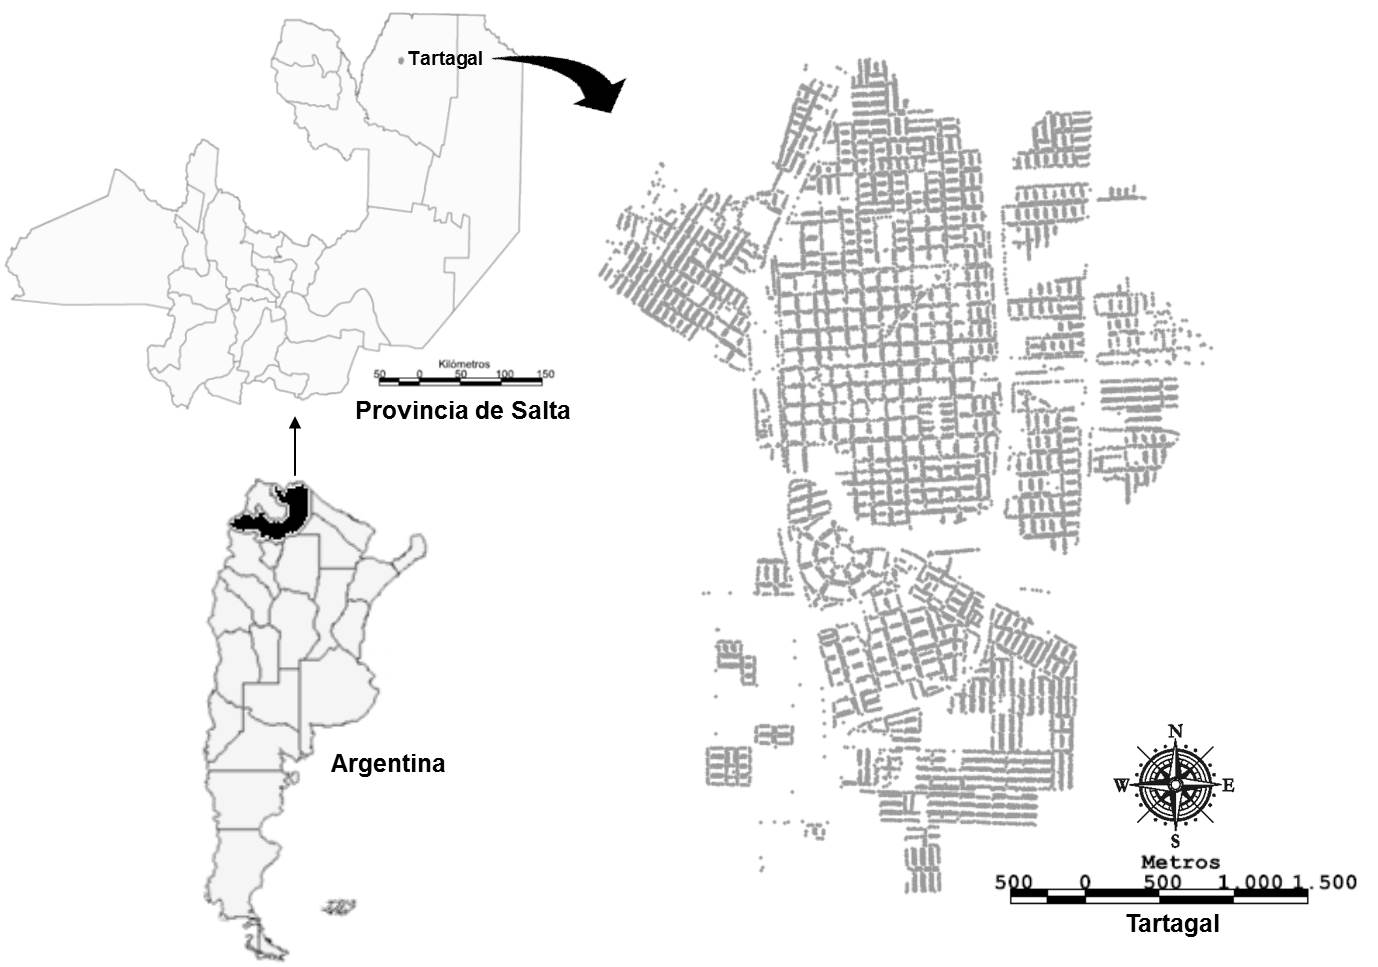
\includegraphics[width=.8\textwidth]{tartagal}
  \end{center}
\end{frame}


\begin{frame}{Obtención y análisis de datos a utilizar}
\begin{itemize}
  \item Oviposición: ovitrampas
  \item De productos satelitales a variables ambientales:
      \begin{itemize}
        \item Propiedades de vegetación: \textbf{NDVI}
        \item Humedad: \textbf{NDWI}
        \item Temperatura de la superficie: \textbf{LST}
        \item Precipitación: \textbf{TRMM}
      \end{itemize}
  \item En todos los casos se contempla un \textit{lag}
\end{itemize}
\end{frame}

\begin{frame}{Obtención y análisis de datos a utilizar}
  Datos de área rural y área urbana
  \begin{center}
    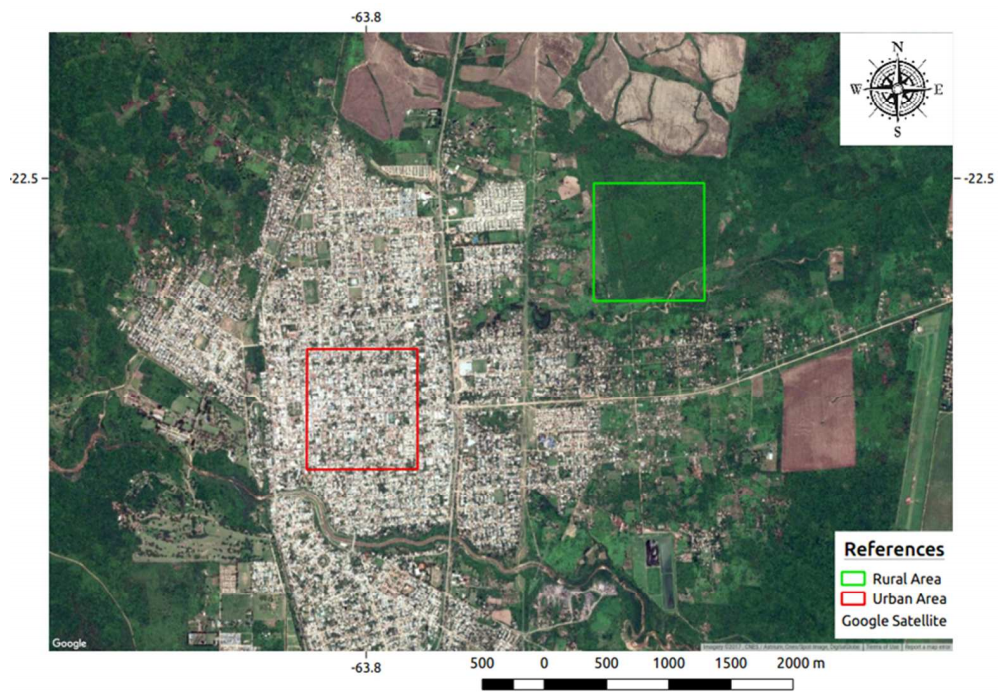
\includegraphics[width=0.7\textwidth]{zones}
  \end{center}
\end{frame}


\begin{frame}{Análisis y selección de datos a utilizar}
\begin{itemize}
  \item Cinco variables elegidas:
    \begin{itemize}
      \item NDVI rural lag 1
      \item NDWI rural lag 1
      \item LST rural dia lag 3
      \item LST rural noche lag 1
      \item TRMM lag 3
    \end{itemize}
    \item Normalización con \textit{z-score}
\end{itemize}
\end{frame}

\begin{frame}{Análisis y selección de datos a utilizar}
  \begin{center}
    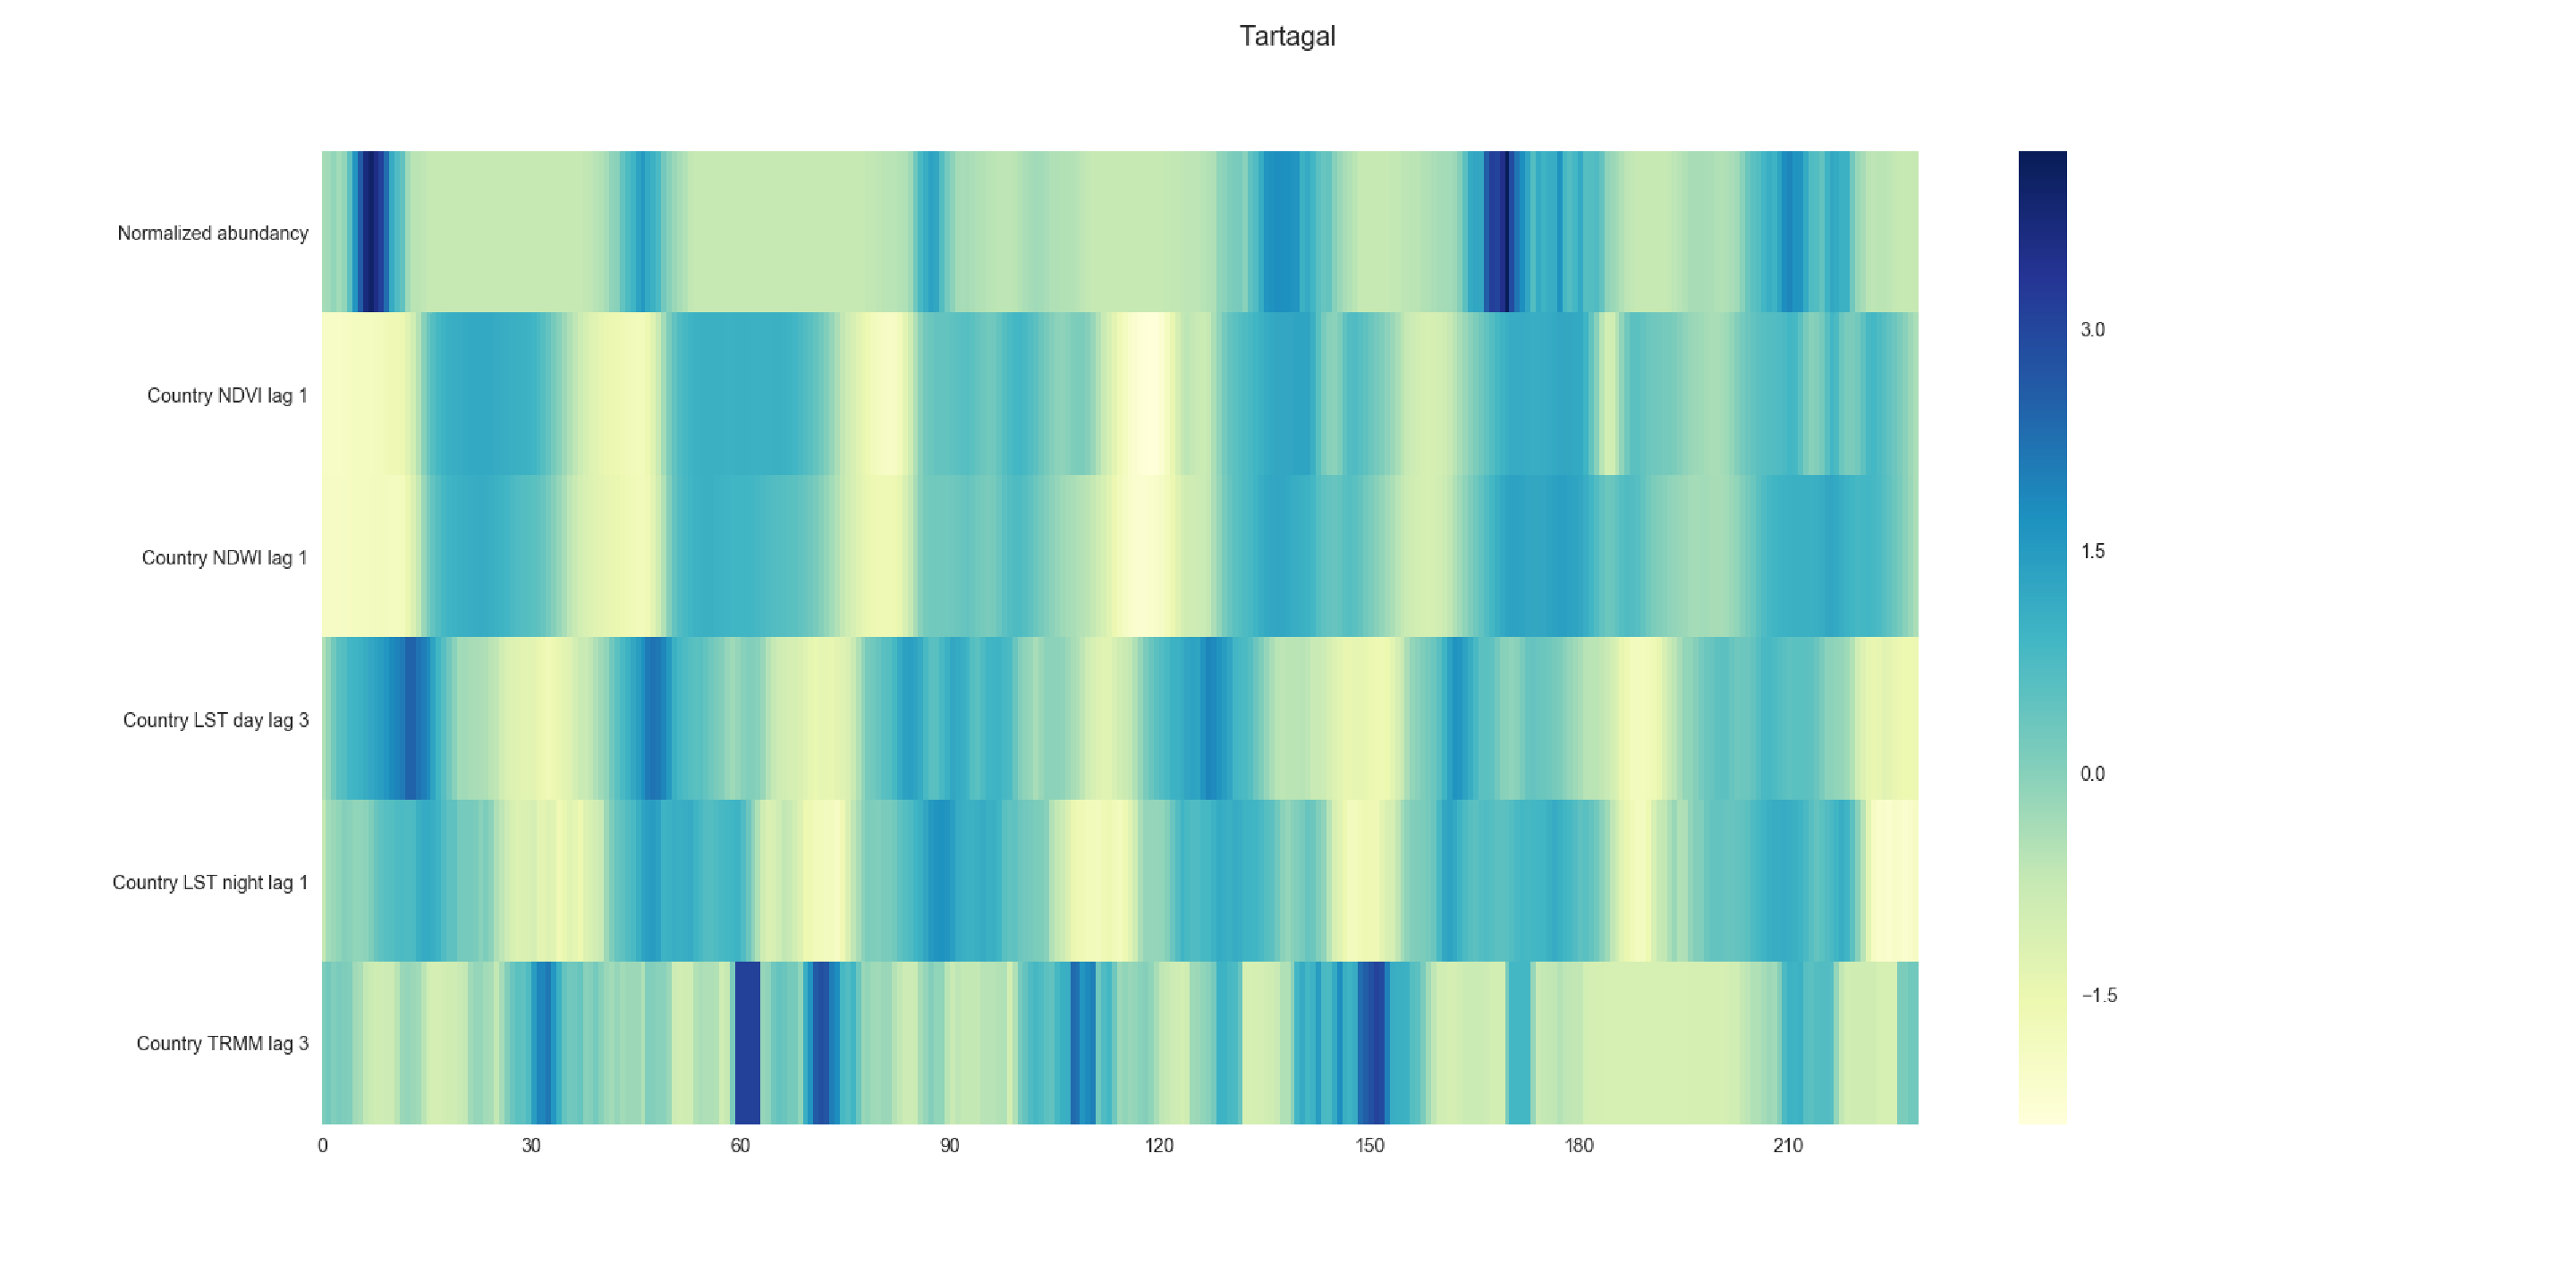
\includegraphics[width=1.22\textwidth]{heatmap}
  \end{center}
\end{frame}


\begin{frame}{Sistema completo}
  \begin{center}
    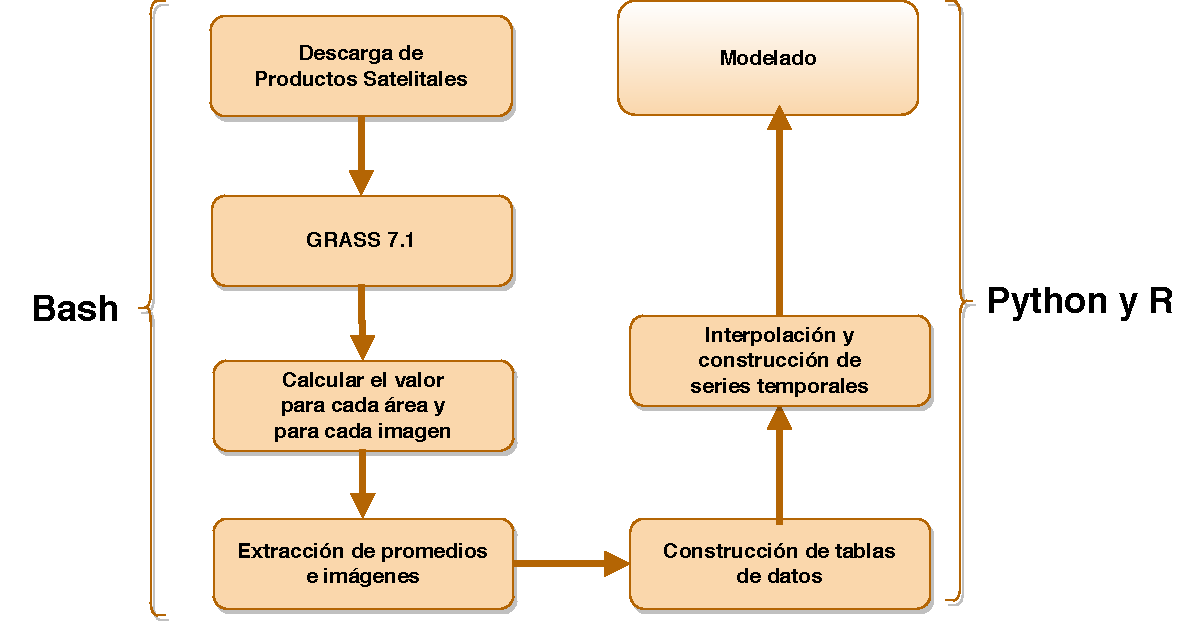
\includegraphics[width=1\textwidth]{sistema_datos}
  \end{center}
\end{frame}


\begin{frame}{Requerimientos de nuestro sistema}
  \begin{itemize}
    \item Facilidad de utilización
    \item Herramienta de limpieza de datos
    \item Flexibilidad para cambiar conjuntos de datos
    \item Herramienta para ajustar hiperparámetros
    \item Generar modelos en formato utilizable en producción
    \item Flexibilidad para agregar nuevos algoritmos
    \item Herramienta de visualización de datos
  \end{itemize}
\end{frame}

\begin{frame}{Arquitectura del sistema}
  \begin{itemize}
    \item Data: \textit{scikit-learn}, \textit{pandas}, \textit{numpy}
    \item Models: \textit{scikit-learn}
    \item Tunning: \textit{Irace} (\textit{Iterated Racing for Automatic Algorithm Configuration})
  \end{itemize}
\end{frame}


\begin{frame}{Modelando poblaciones de mosquito}
  Todos los algoritmos de ML que se utilizaron son de la librería \textit{scikit-learn}
  \begin{itemize}
    \item Lineales:
      \begin{itemize}
        \item Ridge
        \item Tradicional (mínimos cuadrados)
      \end{itemize}
    \item No-lineales:
      \begin{itemize}
        \item Regresión de árboles de decisión (DTR)
        \item Regresión de K-Vecinos más cercanos (KNNR)
        \item Support Vector Regressor (SVR)
        \item Perceptron multicapa (MLP)
      \end{itemize}
  \end{itemize}
\end{frame}



\begin{frame}{Modelando poblaciones de mosquito}
  \begin{center}
    Evaluación y análisis de los modelos generados
  \end{center}
\end{frame}


\begin{frame}{Evaluación y análisis de los modelos generados}
  \begin{center}
    Métodos Lineales
    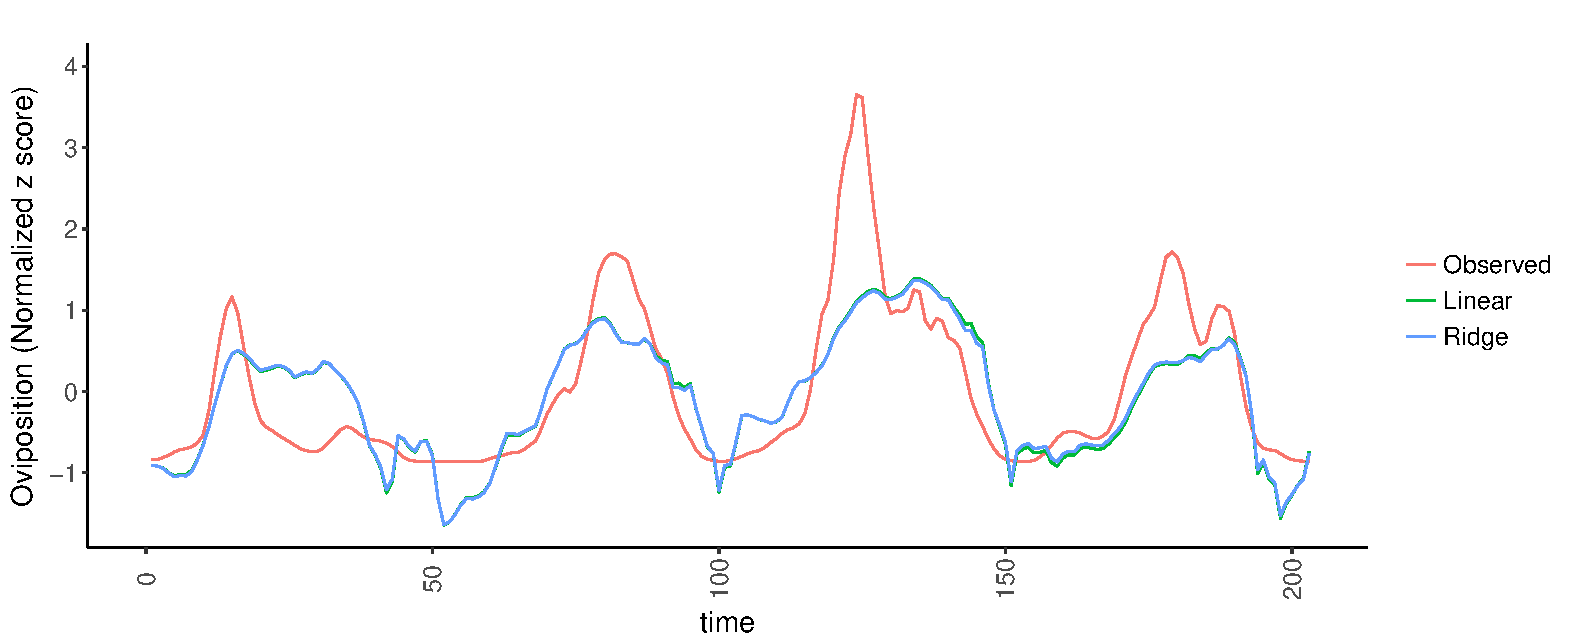
\includegraphics[width=1\textwidth]{RidgeVsTime}
  \end{center}
\end{frame}


\begin{frame}{Evaluación y análisis de los modelos generados}
  \begin{center}
    Regresión de árbol de decisión (DTR)
    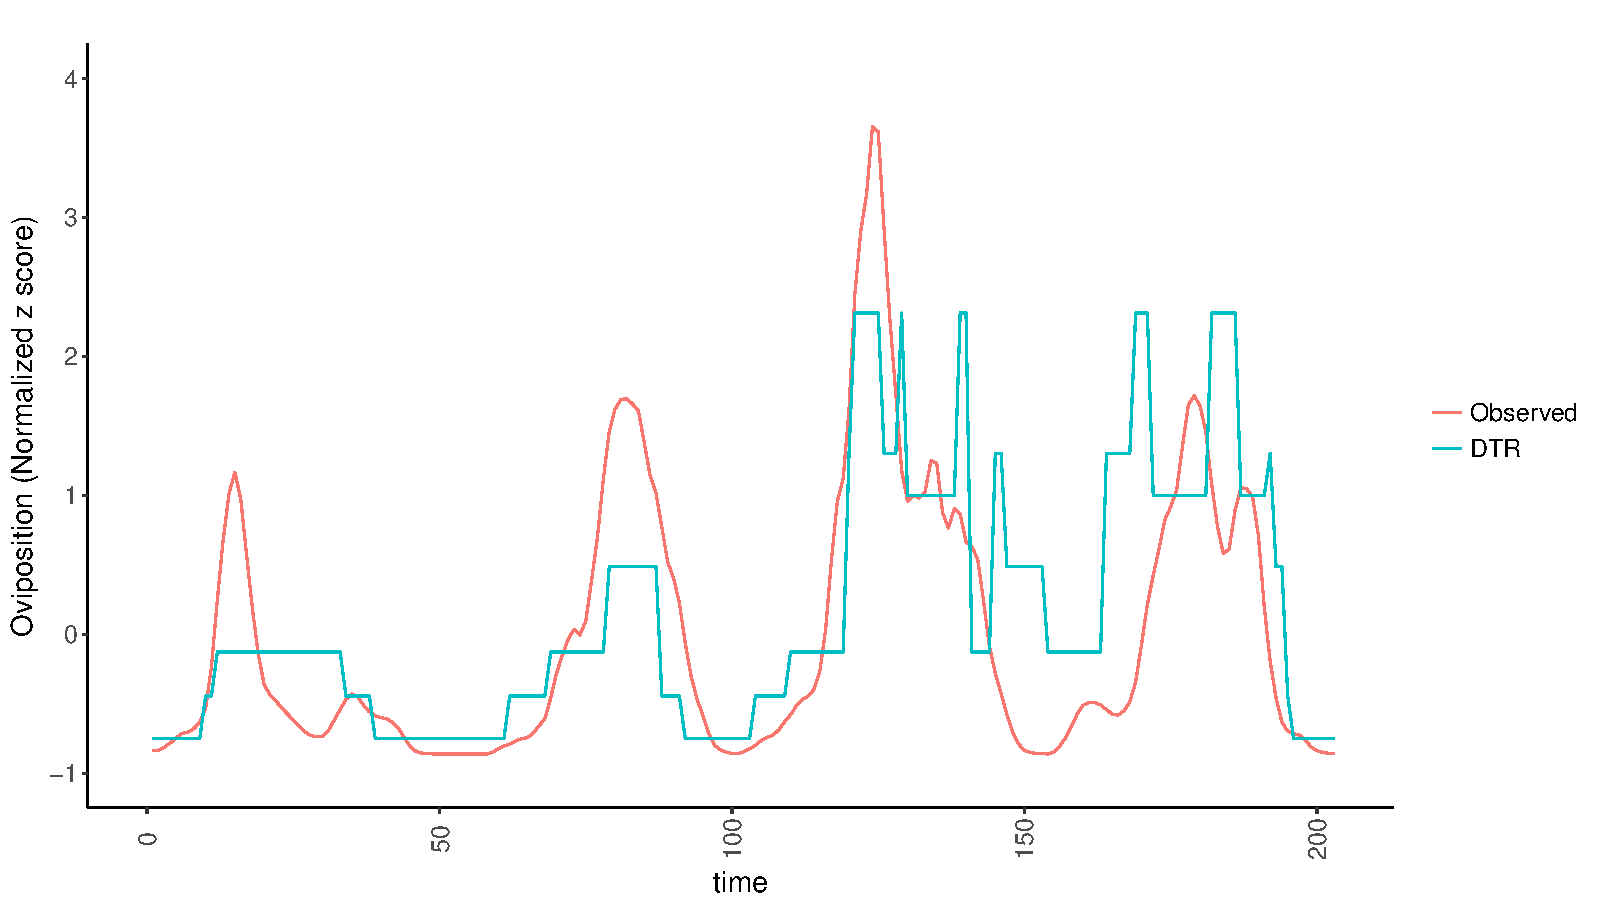
\includegraphics[width=1\textwidth]{dtr}
  \end{center}
\end{frame}


\begin{frame}{Evaluación y análisis de los modelos generados}
  \begin{center}
    Regresión de K-Vecinos más cercanos (KNNR)
    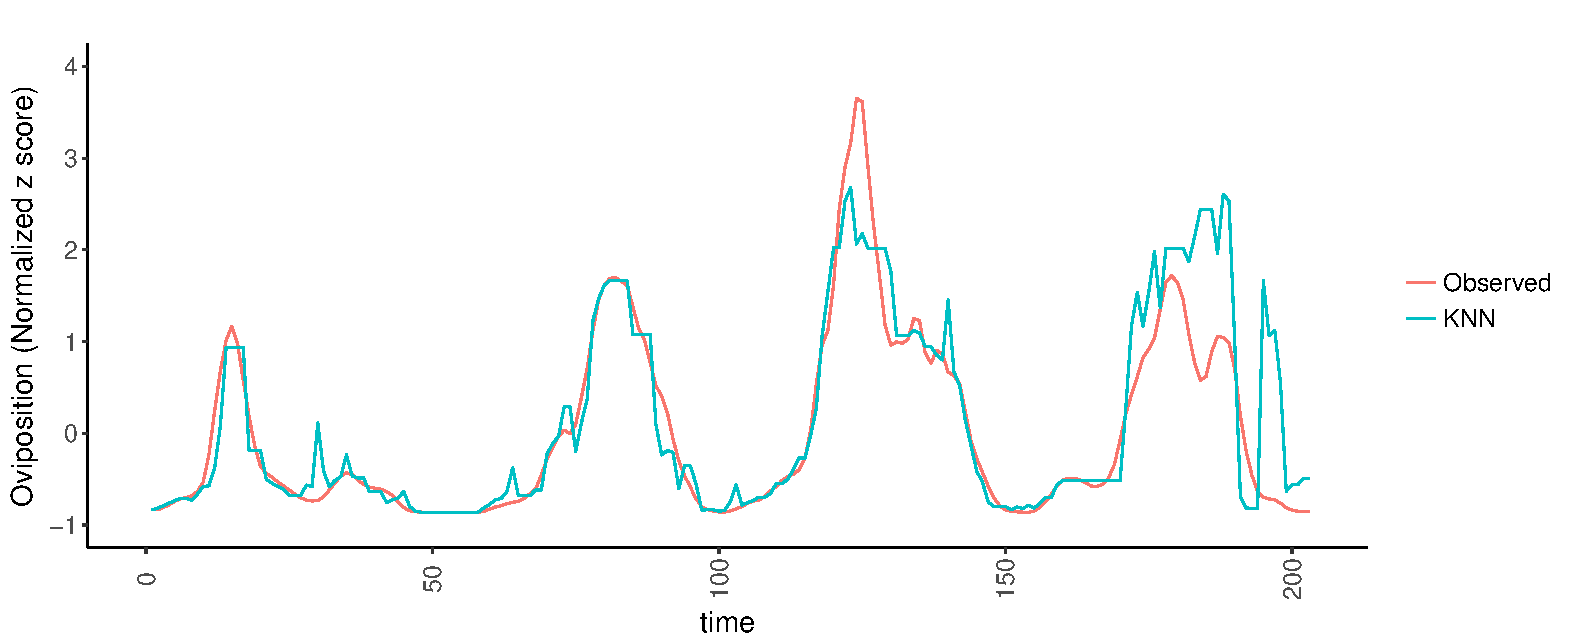
\includegraphics[width=1\textwidth]{knn}
  \end{center}
\end{frame}


\begin{frame}{Evaluación y análisis de los modelos generados}
  \begin{center}
    Support Vector Regressor (SVR)
    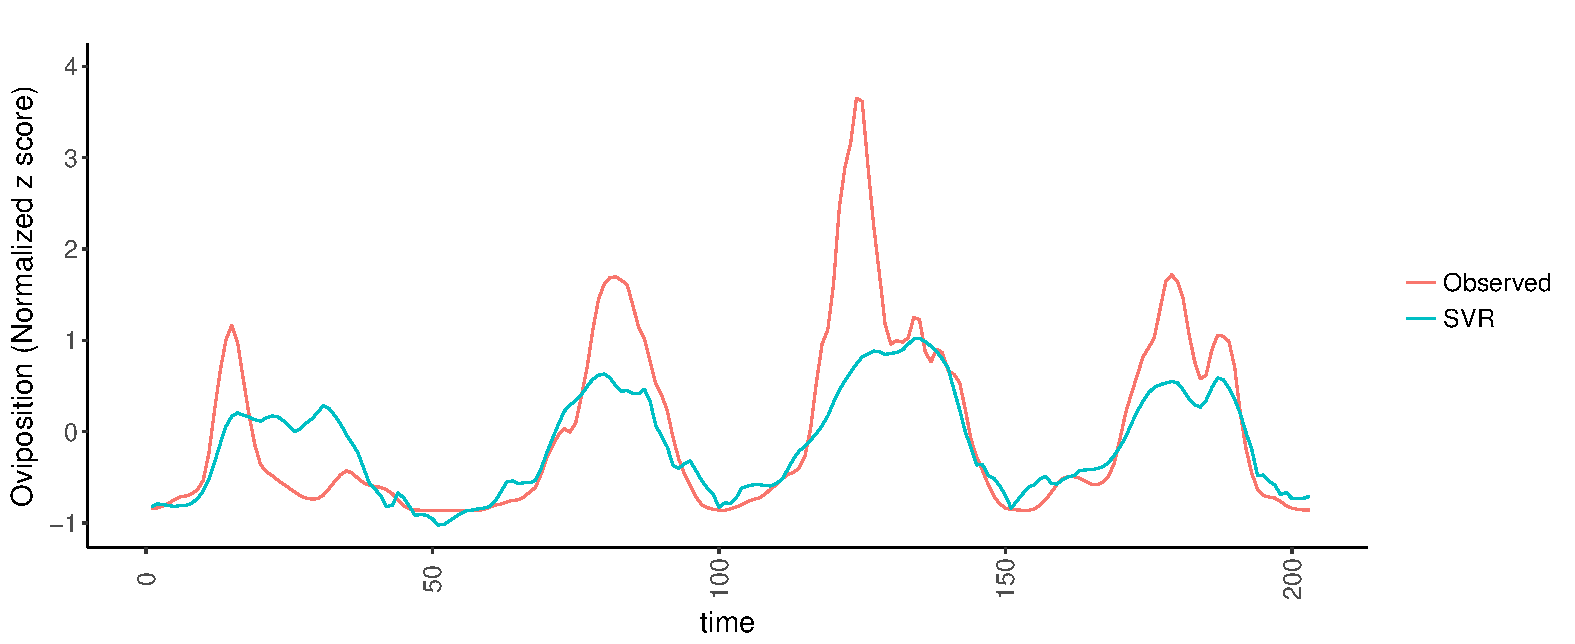
\includegraphics[width=1\textwidth]{svr}
  \end{center}
\end{frame}



\begin{frame}{Evaluación y análisis de los modelos generados}
  \begin{center}
    Perceptron multicapa (MLP)
    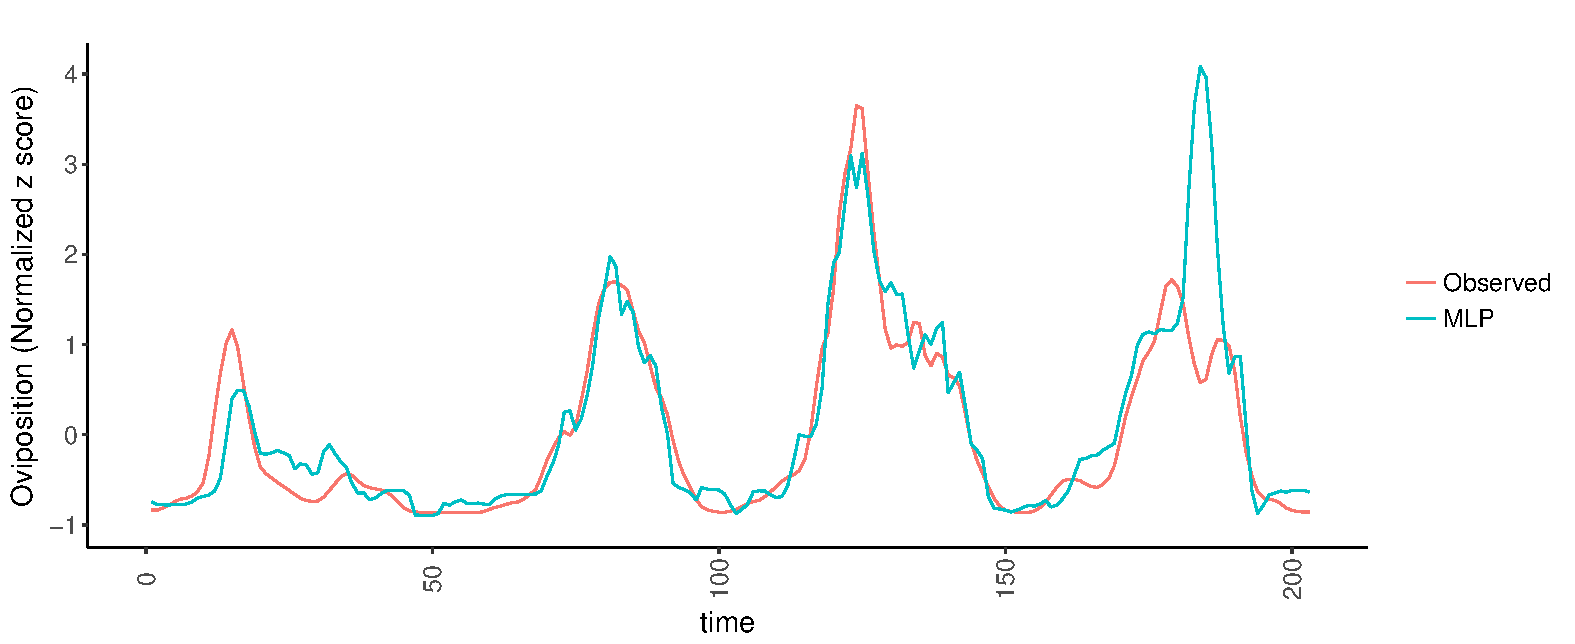
\includegraphics[width=1\textwidth]{mlp}
  \end{center}
\end{frame}




\begin{frame}{Evaluación y análisis de los modelos generados}

%\begin{table}[hbt]
\centering
Resumen de los datos observados y los ajustados
%\caption{Resumen de los datos observados y los ajustados}\label{Tab:Summary}
\begin{tabular}{*7{r}}
\toprule
&Mín	&$q_{1/4}$	&$q_{1/2}$	&Media	&$q_{3/4}$	&Máx\\ \cmidrule(lr){2-7}
Observado	&$-0.863$	&$-0.742$	&$-0.487$	&$0.000$	&$0.704$	&$3.652$\\
Lineal	&$-1.641$	&$-0.716$	&$ 0.027$	&$-0.087$	&$0.462$	&$1.387$\\
Ridge	&$-1.638$	&$-0.680$	&$ 0.028$	&$-0.084$	&$0.459$	&$1.370$\\
MLP	&$-0.894$	&$-0.677$	&$-0.323$	&$0.093$	&$0.716$	&$4.084$\\
DTR	&$-0.752$	&$-0.752$	&$-0.128$	&$0.138$	&$0.998$	&$2.312$\\
KNNR	&$-0.863$	&$-0.699$	&$-0.501$	&$0.099$	&$1.033$	&$2.679$\\
SVR	&$-1.021$	&$-0.601$	&$-0.232$	&$-0.147$	&$0.309$	&$1.023$\\
\bottomrule
\end{tabular}
%\end{table}
\end{frame}



\begin{frame}{Evaluación y análisis de los modelos generados}
  \begin{center}
    Scatterplot de datos observados vs datos predichos
    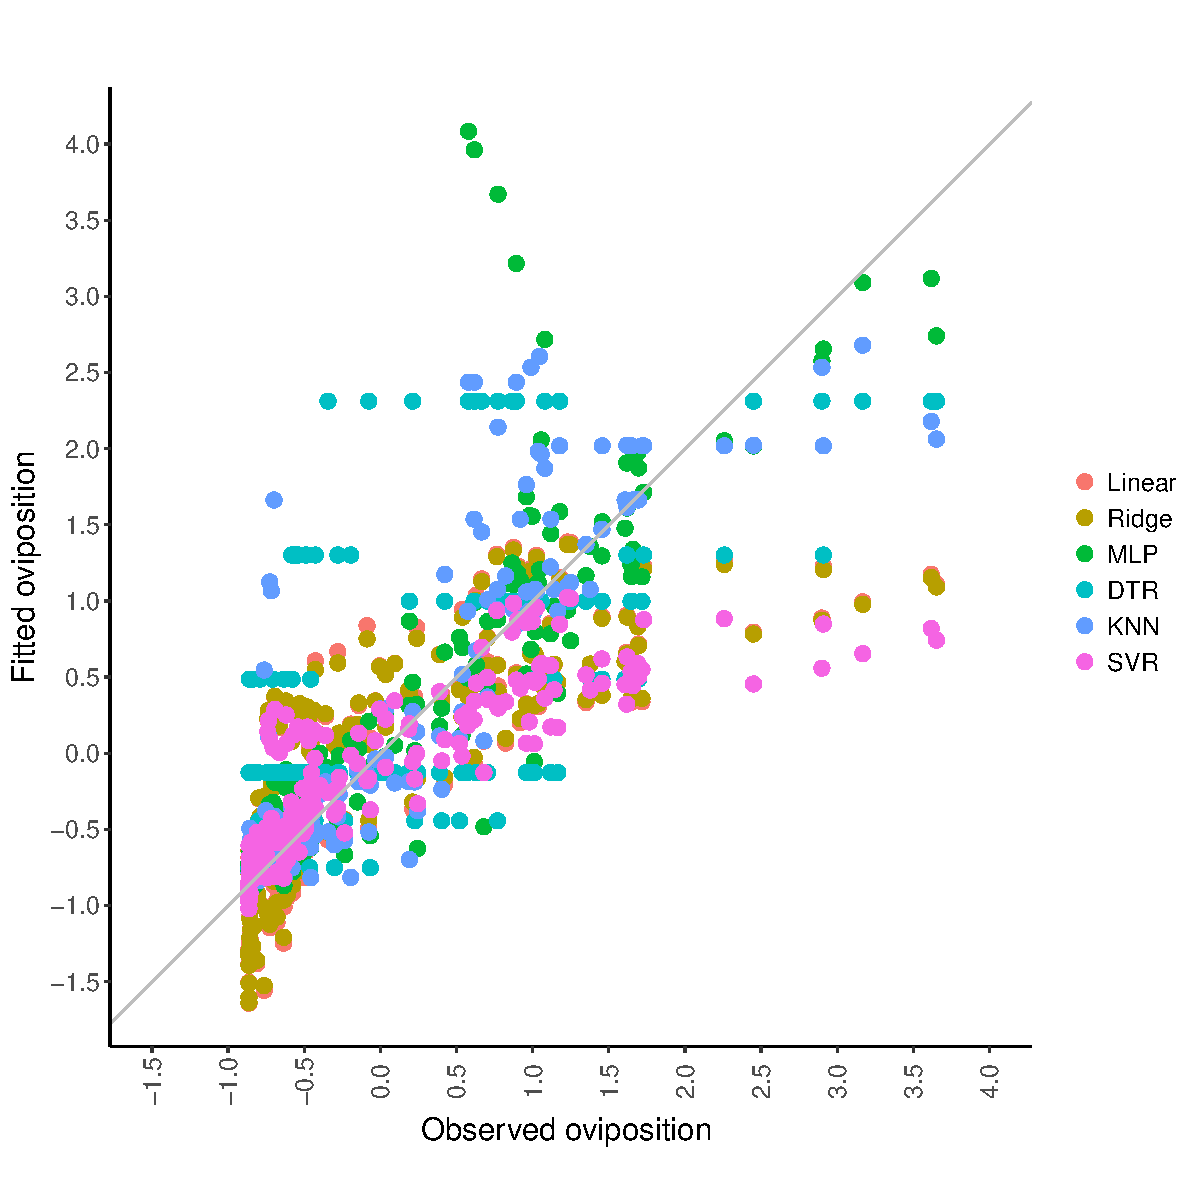
\includegraphics[width=0.6\textwidth]{scatterplot}
  \end{center}
\end{frame}




\begin{frame}{Evaluación y análisis de los modelos generados}
  \begin{center}
    Discusión de resultados obtenidos
  \end{center}
\end{frame}


\begin{frame}{Fin}
  \begin{center}
    Gracias! \\ Preguntas?
  \end{center}
\end{frame}


\begin{frame}{Referencias}
  \begin{itemize}
    \item https://github.com/juansca/WordVectors

  \end{itemize}
\end{frame}








\appendix

\end{document}

%% \begin{frame}{Blocks}
%%   Three different block environments are pre-defined and may be styled with an
%%   optional background color.

%%   \begin{block}{Default}
%%     Block content.
%%   \end{block}

%%   \begin{alertblock}{Alert}
%%     Block content.
%%   \end{alertblock}

%%   \begin{exampleblock}{Example}
%%     Block content.
%%   \end{exampleblock}
%%   \stepcounter{beamerpauses}
%%   \begin{itemize}[<+->]
%%     \item Hola
%%     \item Chau
%%   \end{itemize}
%% \end{frame}
